%!TEX root =../mapp-challenge-18-game-book.tex
% ^ leave for LaTeXTools build functionality

\phChapterWorksheet{Blind Luck}{Cryptic Puzzle 3}

The Nickname Rater suggests you continue your journey down Road \(500\%\),
where an elusive \textbf{Dojo Master} is known to battle up-and-coming trainers.
You arrive at the dojo, but it seems that a secret password is required to
enter, and your only clue is the following image.

\begin{center}
  RED BLUE YELLOW GOLD SILVER CRYSTAL

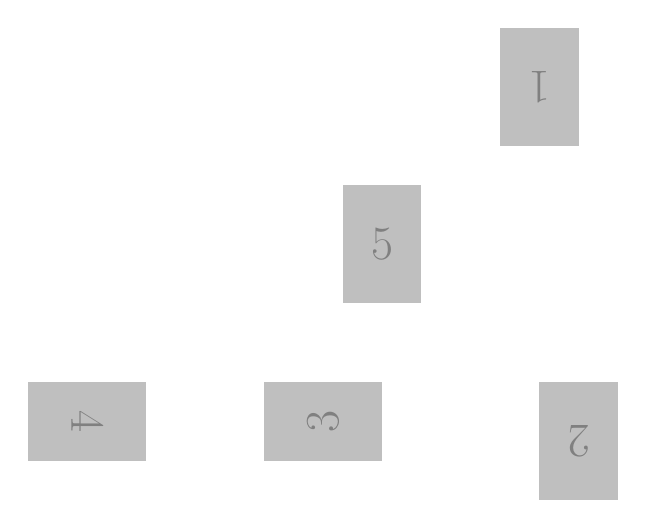
\begin{tikzpicture}[x=0.5cm,y=0.5cm]
  \fill[color=lightgray] (8,14) rectangle (10,17);
  \fill[color=lightgray] (0,10) rectangle (3,12);
  \fill[color=lightgray] (6,10) rectangle (9,12);
  \fill[color=lightgray] (13,9) rectangle (15,12);
  \fill[color=lightgray] (12,18) rectangle (14,21);

  \blindCrissCrossEntry{(0,0)}{(3,12)};
  \blindCrissCrossEntry{(2,9)}{(16,12)};
  \blindCrissCrossEntry{(10,5)}{(13,11)};
  \blindCrissCrossEntry{(7,9)}{(10,17)};
  \blindCrissCrossEntry{(0,16)}{(12,19)};
  \blindCrissCrossEntry{(11,15)}{(14,23)};

  \node at (9,15.5) {\LARGE\rotatebox{0}{\textcolor{gray}{5}}};
  \node at (1.5,11) {\LARGE\rotatebox{-90}{\textcolor{gray}{4}}};
  \node at (7.5,11) {\LARGE\rotatebox{90}{\textcolor{gray}{3}}};
  \node at (14,10.5) {\LARGE\rotatebox{180}{\textcolor{gray}{2}}};
  \node at (13,19.5) {\LARGE\rotatebox{180}{\textcolor{gray}{1}}};
\end{tikzpicture}
\end{center}

You'd move the \textbf{sun and moon} to figure out that password and battle the
Dojo Master! Calmly, you \textbf{shut your eyes} and begin to ponder the
solution to this mystery...


% Include below for aucTeX integration
%%% Local Variables:
%%% mode: latex
%%% TeX-master: "../mapp-challenge-18-game-book"
%%% End:
